\subsection{\Wb-boson production in \RunpPb at 8.16 TeV} \label{sec:WBoson_Results_Observables}

The \WToMuNupm differential cross sections are derived using \eq{eq:CrossSection}. The results of the differential cross sections of \WToMuNuPl and \WToMuNuMi are shown as a function muon \etaMuCM in \fig{fig:CrossSection_WToMu_PA}. The vertical error bars represent the statistical uncertainties from the number of \WToMuNu events measured in each \etaMuCM range, while the brackets show the statistical and total systematic uncertainties summed in quadrature. The global integrated luminosity uncertainty of {3.5\%}~\cite{LUM-17-002} is not shown in the figures.

\begin{figure}[htb!]
 \centering
 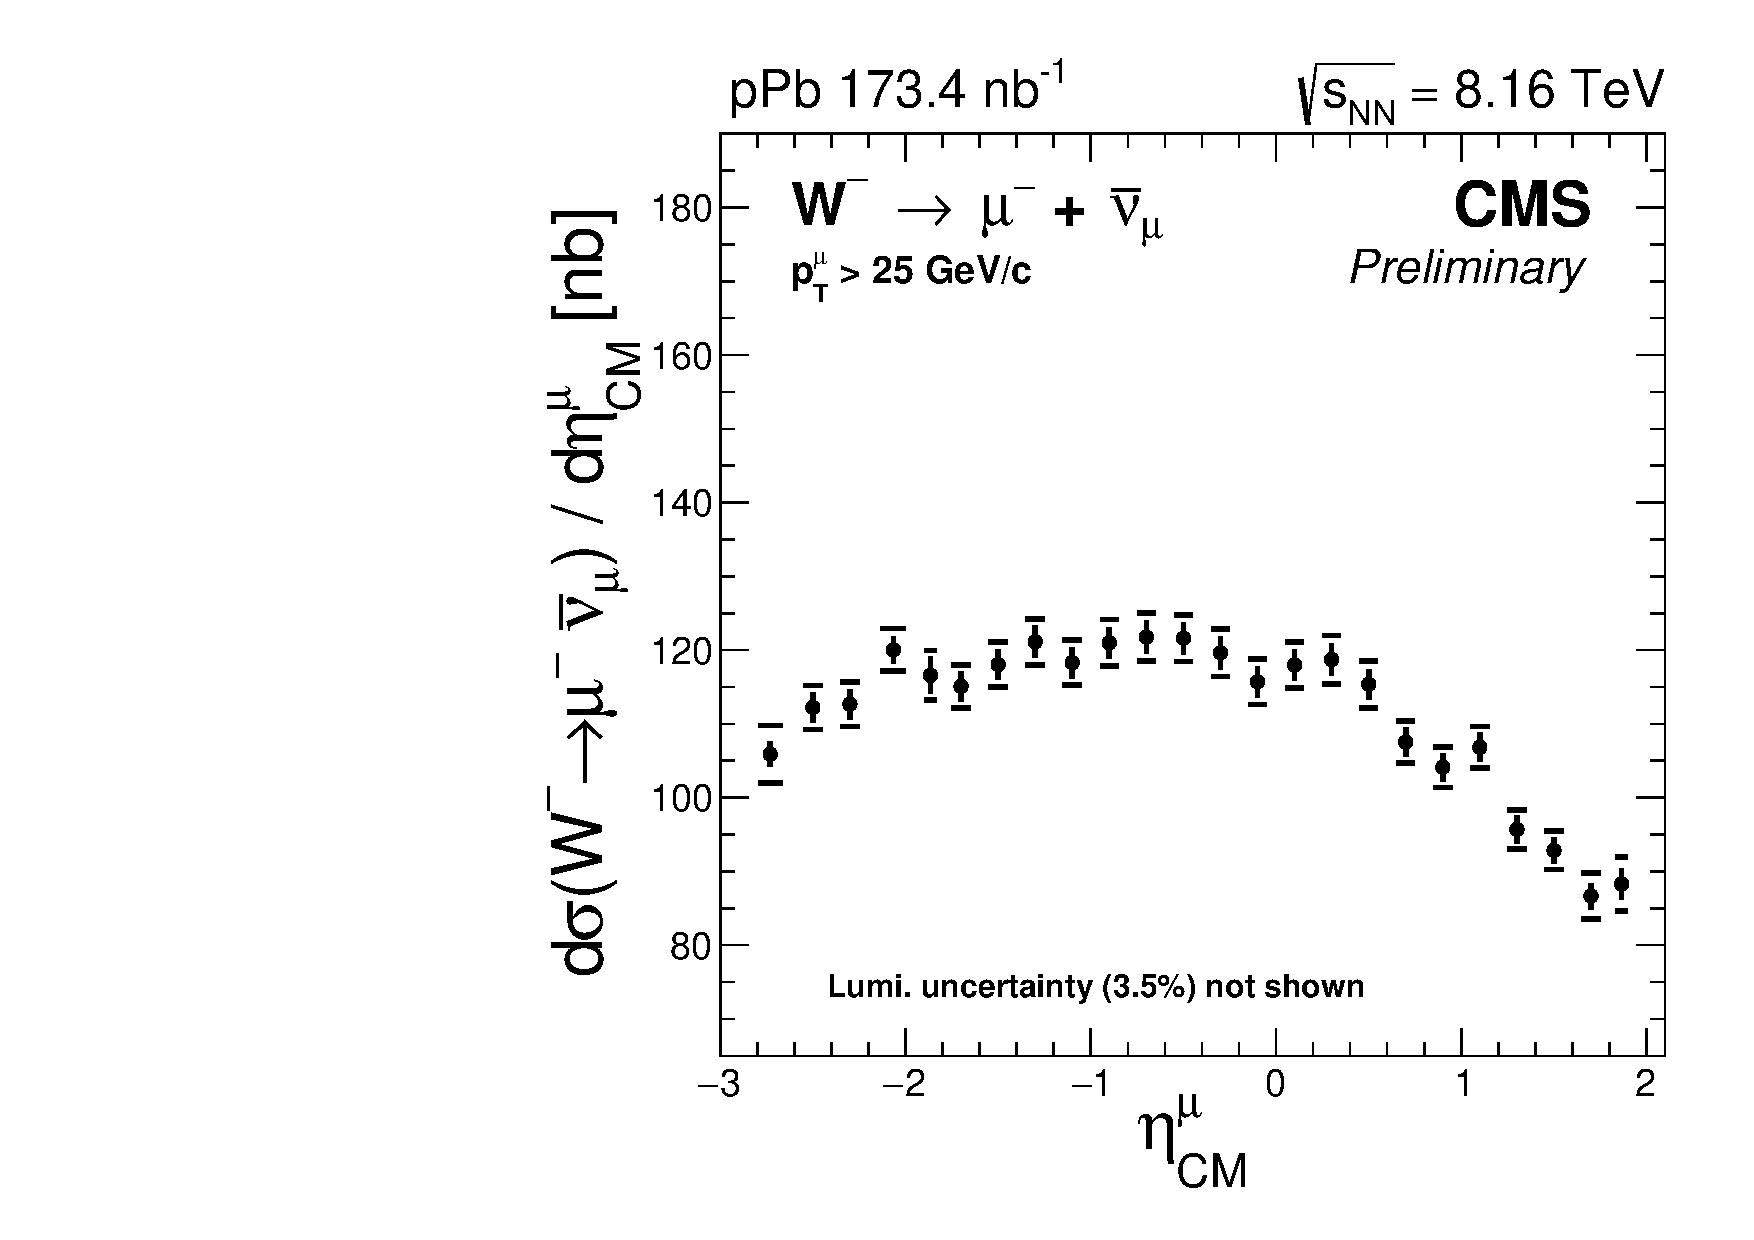
\includegraphics[width=0.45\textwidth]{Figures/WBoson/Results/DATA/gr_WToMuMi_PA_Cross_Section_EffTnP_Nominal.pdf}
%%
 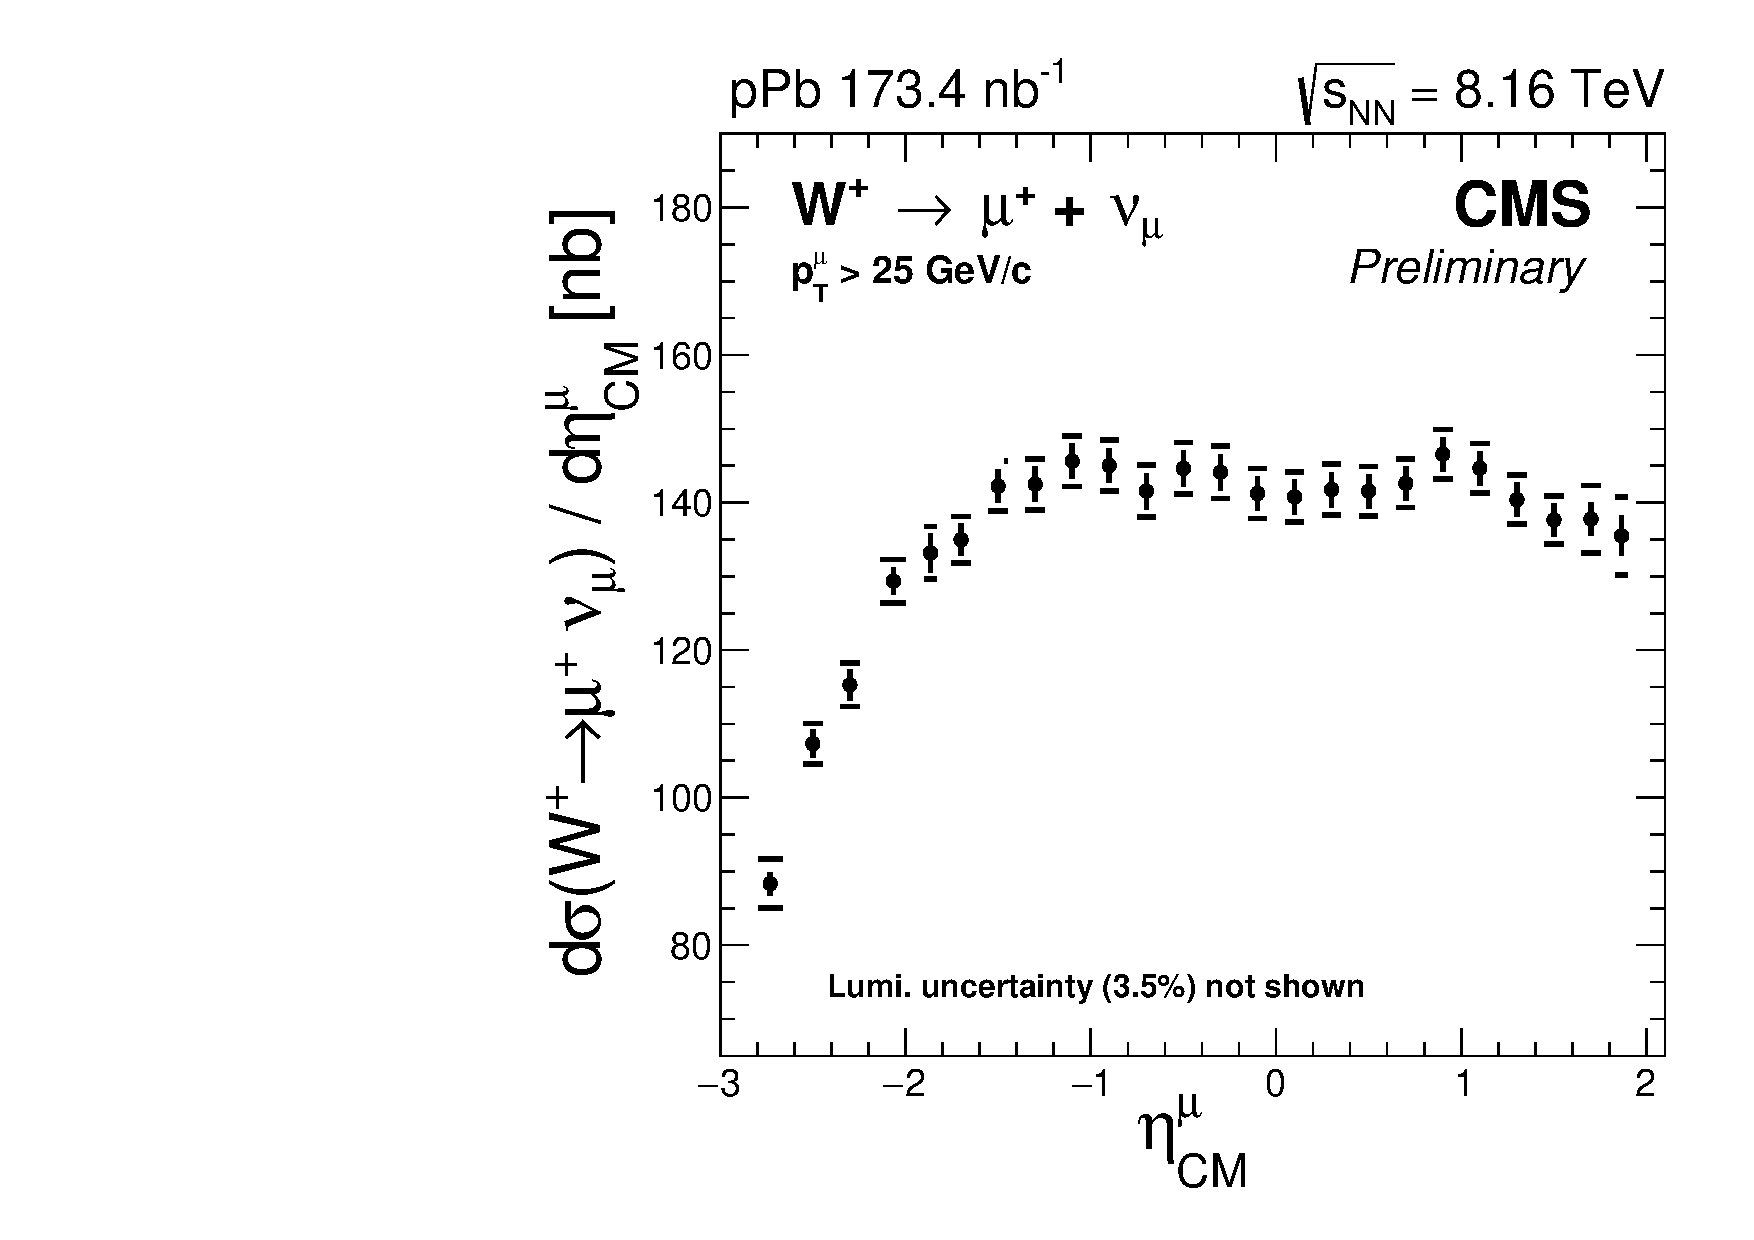
\includegraphics[width=0.45\textwidth]{Figures/WBoson/Results/DATA/gr_WToMuPl_PA_Cross_Section_EffTnP_Nominal.pdf}
 \caption{Differential production cross sections for \WToMuNuPl (left) and \WToMuNuMi (right), as a function of the muon pseudorapidity in the center-of-mass frame. The brackets represent the statistical and systematic uncertainties summed in quadrature, while the error bars show the statistical uncertainties only. The global luminosity uncertainty of 3.5\%~\cite{LUM-17-002} is not shown. }
 \label{fig:CrossSection_WToMu_PA}
\end{figure}

The opposite trend seen between the \WToMuNuPl and \WToMuNuMi differential cross sections as a function of \etaMuCM is expected from parity violation of the electroweak interaction. The \Wp bosons decay to a right-handed anti-muon boosted in the opposite direction, while the \Wm bosons decay to a left-handed muon along the direction of the \Wm boson.

The muon charge asymmetry is determined from the efficiency-corrected signal event yields using \eq{eq:MuonChargeAsymmetry}. The measured muon charge asymmetry is shown in \fig{fig:ChargeAsymmetry_WToMu_PA} as a function muon $\etaMuCM$.

\begin{figure}[htb!]
 \centering
 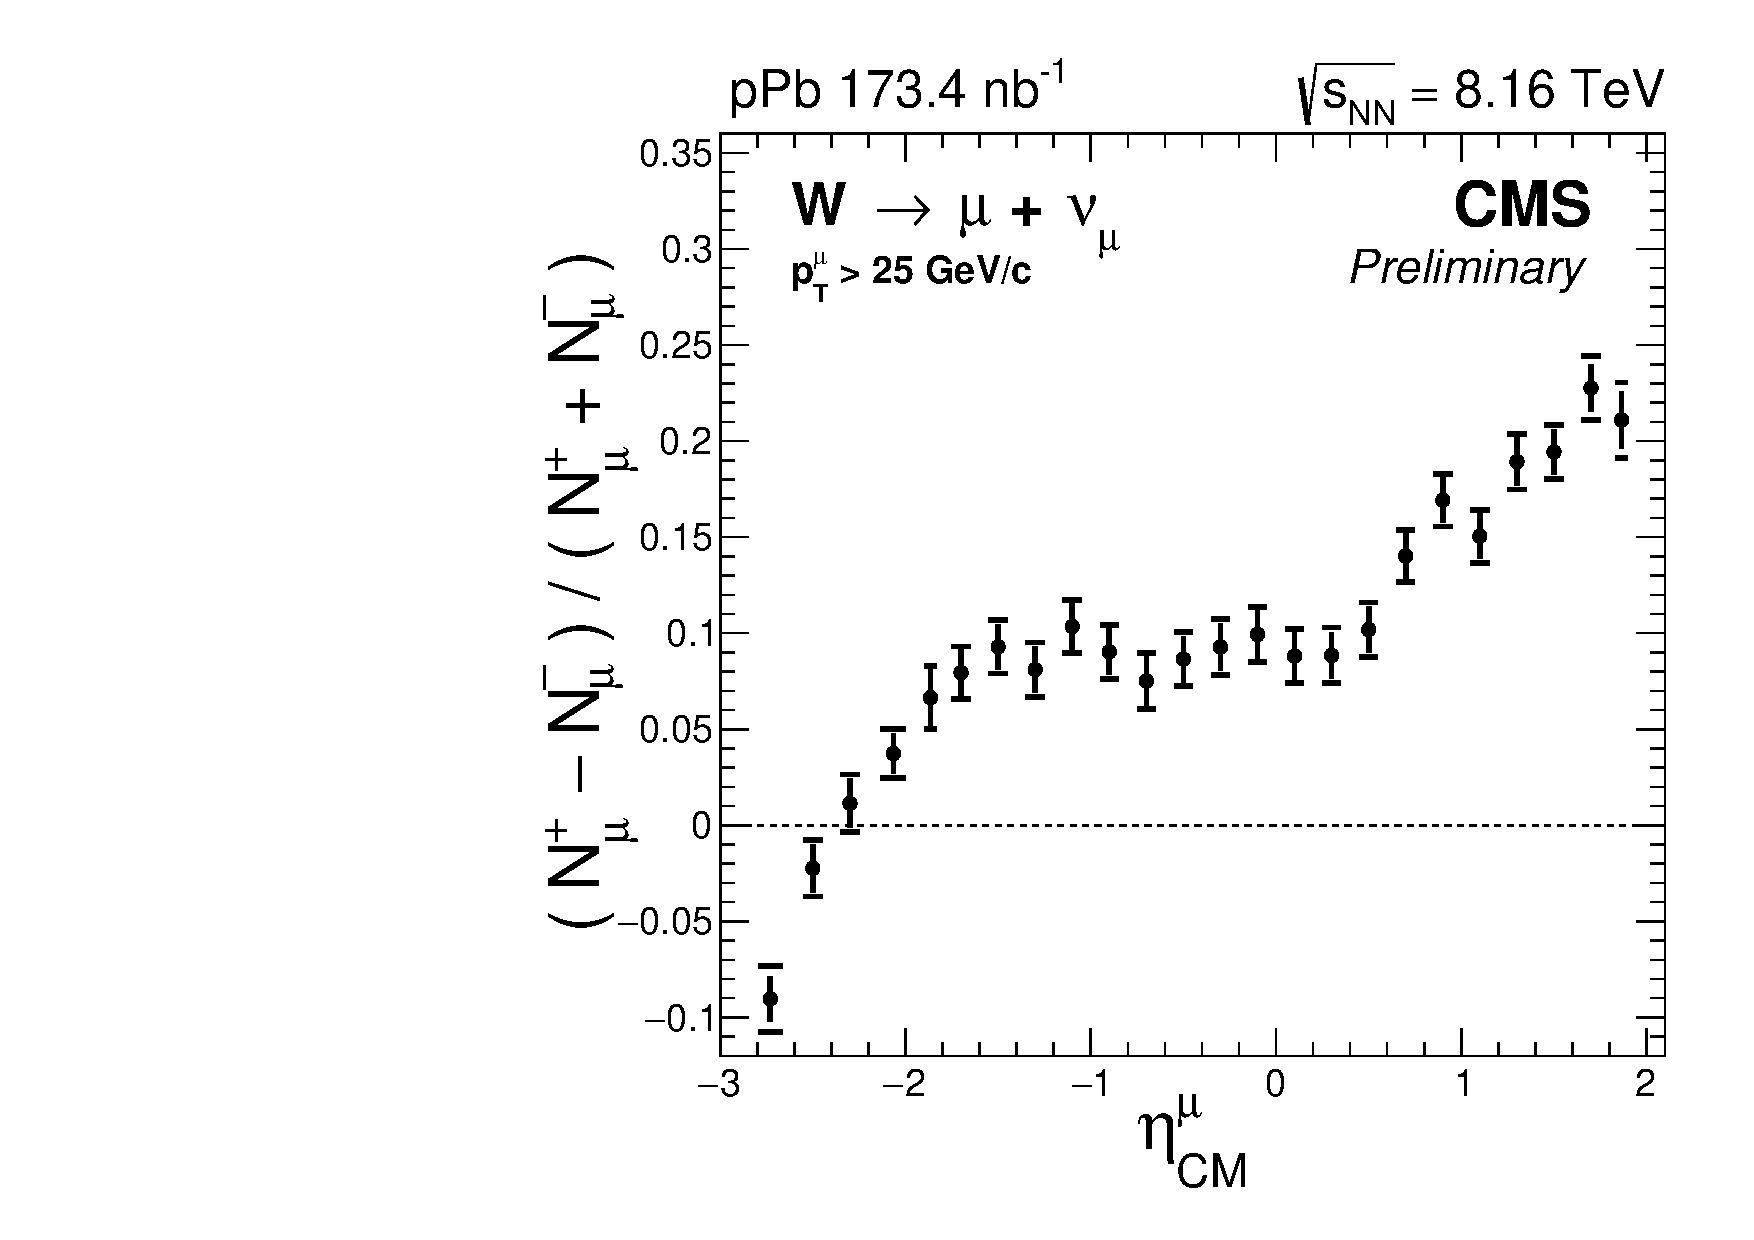
\includegraphics[width=0.55\textwidth]{Figures/WBoson/Results/DATA/gr_WToMuInc_PA_Charge_Asymmetry_EffTnP_Nominal.pdf}
 \caption{Muon charge asymmetry as a function of the muon pseudorapidity in the center-of-mass frame. The brackets represent the statistical and systematic uncertainties summed in quadrature, while the error bars show the statistical uncertainties only.}
 \label{fig:ChargeAsymmetry_WToMu_PA}
\end{figure}

The \WToMuNuPl and \WToMuNuMi forward-backward ratios are computed using \eq{eq:MuonForwardBackwardAsymmetryCharged}, while the charge-summed forward-backward ratio is determined using \eq{eq:MuonForwardBackwardAsymmetry}. As mentioned in \sect{sec:WBoson_Analysis_Samples_Data}, the forward region ($\etaMuCM > 0$) is defined on the proton-going direction while the backward region corresponds to the Pb-going direction. The results of the muon forward-backward ratios are shown in \fig{fig:ForwardBackwardRatio_WToMu_PA}.

\begin{figure}[htb!]
 \centering
 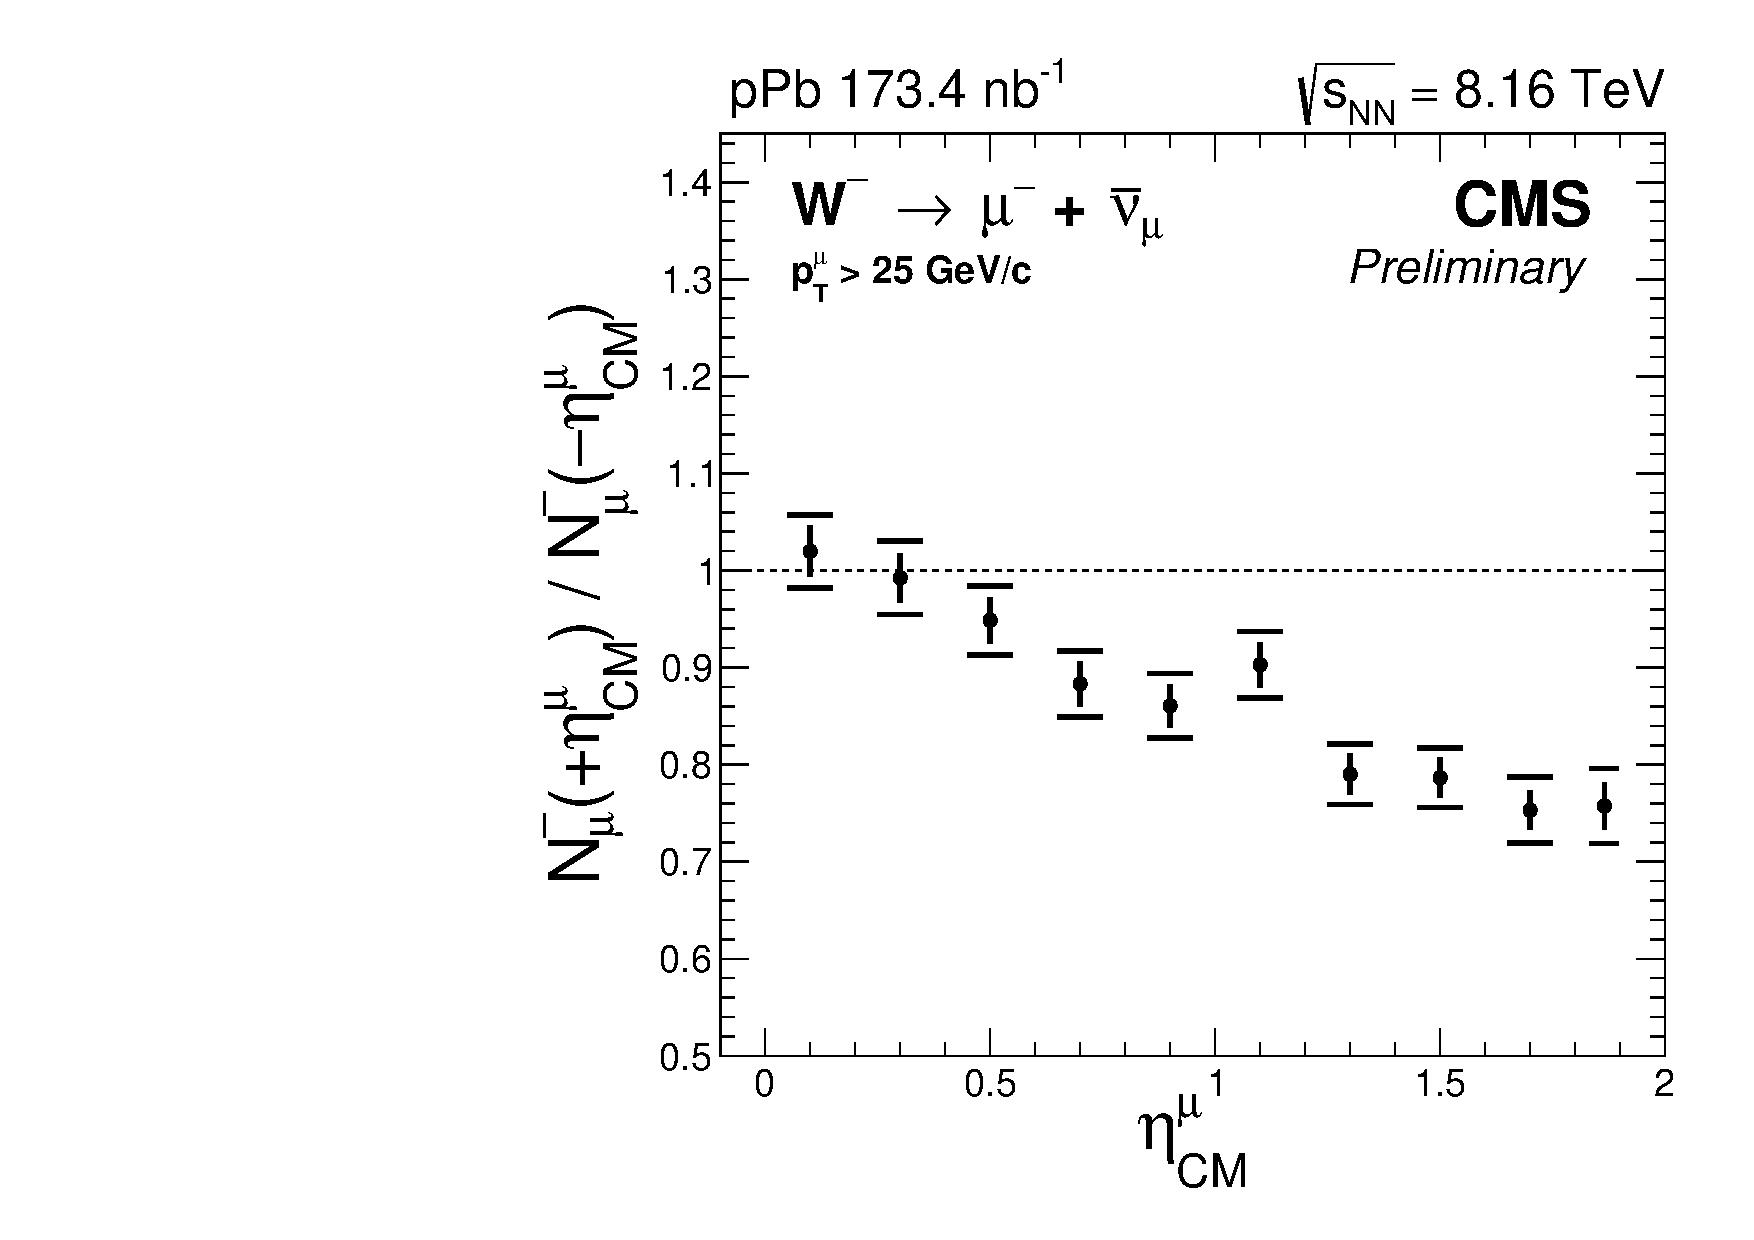
\includegraphics[width=0.45\textwidth]{Figures/WBoson/Results/DATA/gr_WToMuMi_PA_ForwardBackward_Ratio_EffTnP_Nominal}
%%
 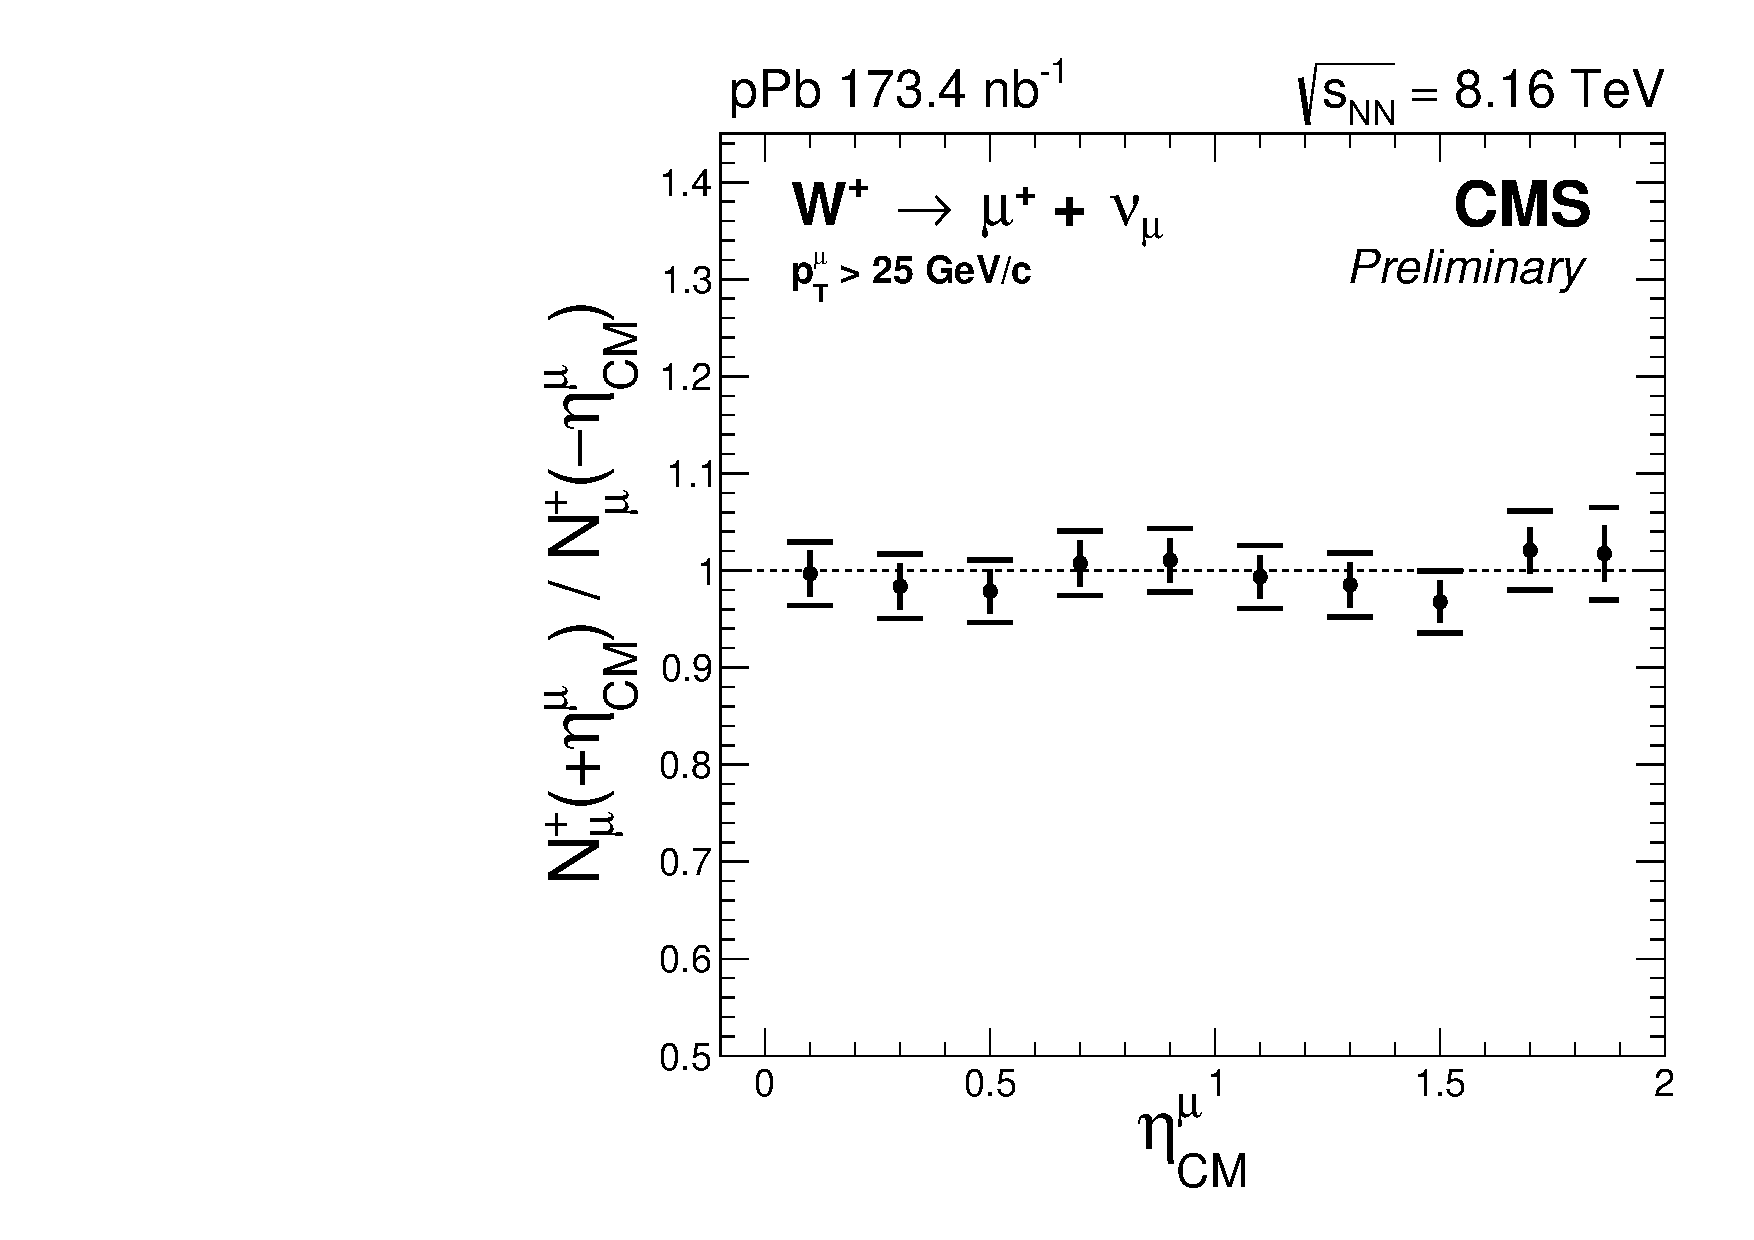
\includegraphics[width=0.45\textwidth]{Figures/WBoson/Results/DATA/gr_WToMuPl_PA_ForwardBackward_Ratio_EffTnP_Nominal}
%%
 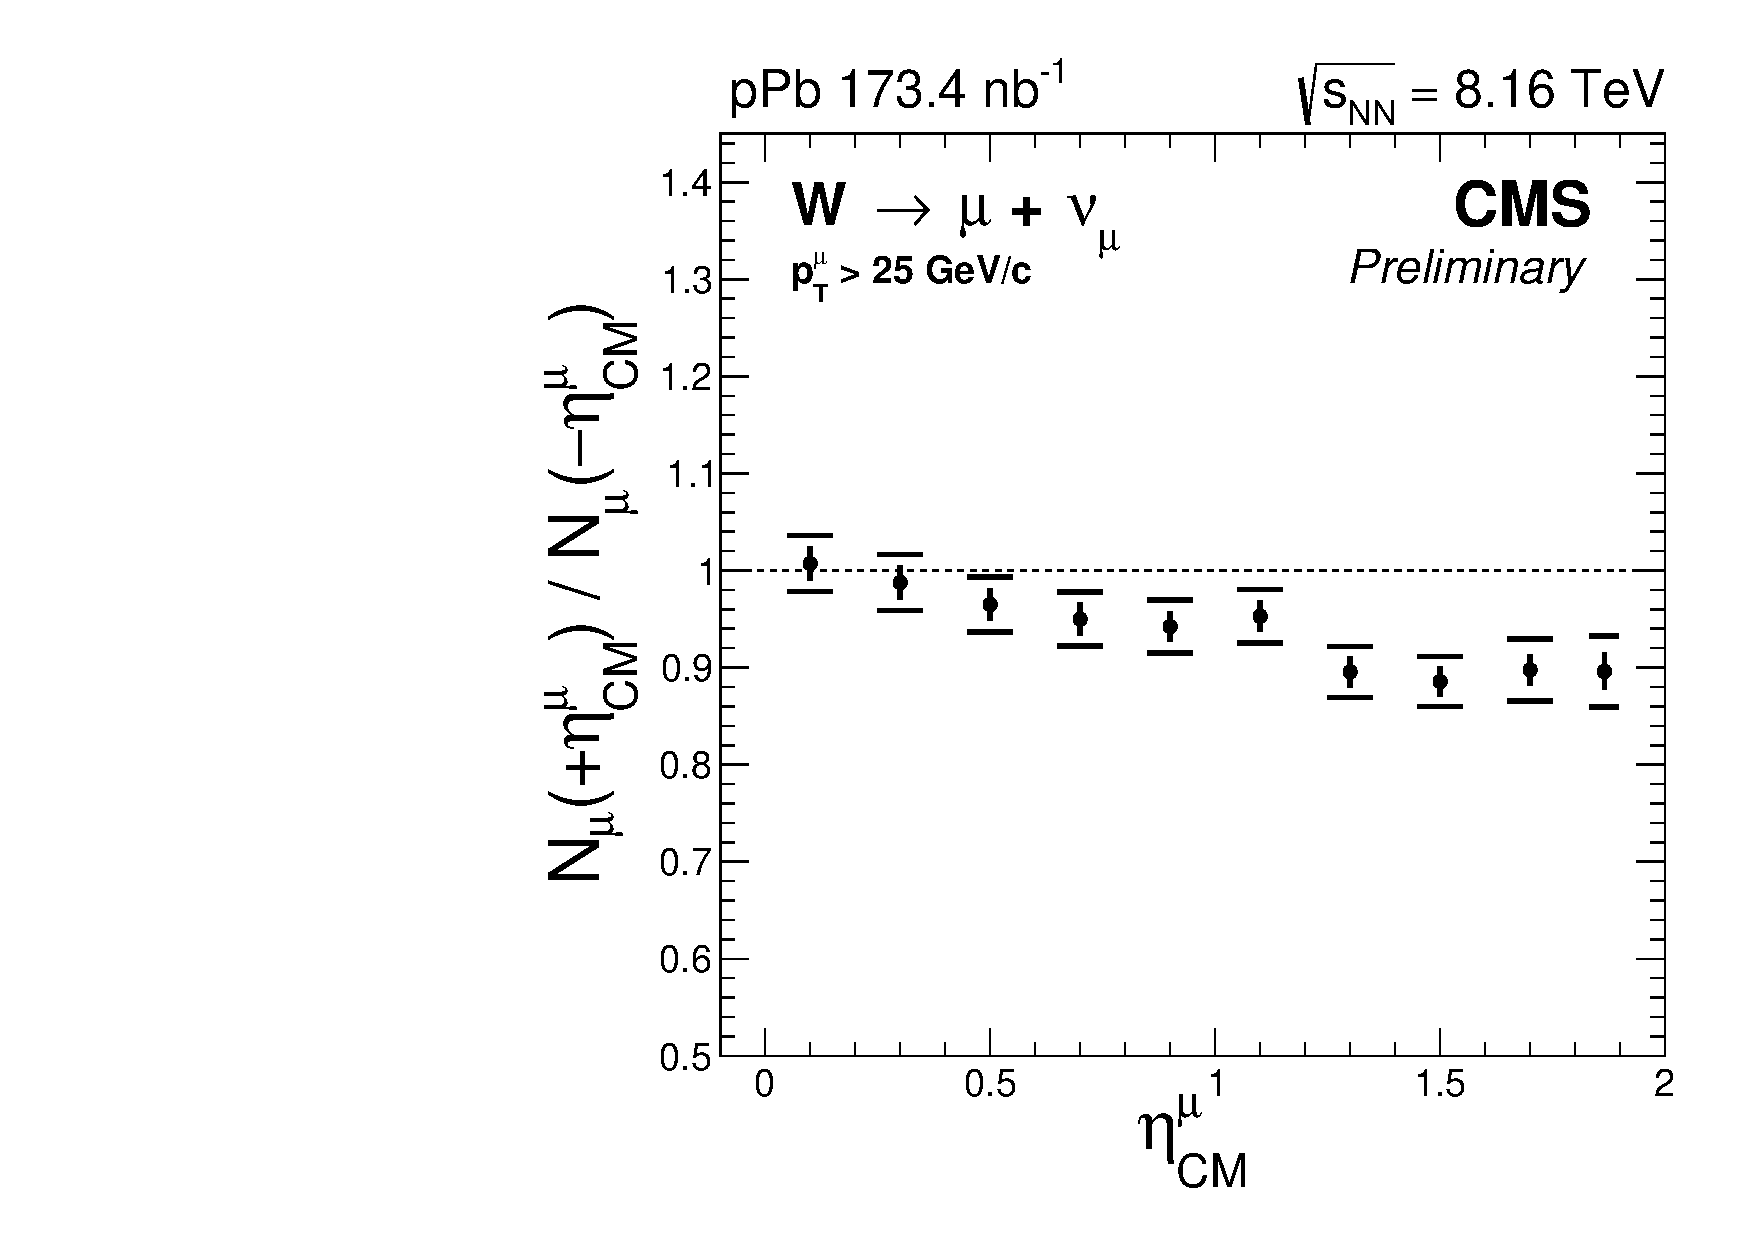
\includegraphics[width=0.45\textwidth]{Figures/WBoson/Results/DATA/gr_WToMuInc_PA_ForwardBackward_Ratio_EffTnP_Nominal}
 \caption{Forward-backward ratios, for the positive (top-left), negative (top-right) and all (bottom) charged muons. The brackets represent the statistical and systematic uncertainties summed in quadrature, while the error bars show the statistical uncertainties only.}
 \label{fig:ForwardBackwardRatio_WToMu_PA}
\end{figure}

% END OF SUBSECTION